% chapter1.tex
\chapter{Hàm số}
\label{ch:intro}

\section{Tính đơn điệu của hàm số}

\begin{lythuyetbox}{Lý thuyết căn bản}

Cho hàm số $y = f(x)$ xác định trên khoảng $K$.
Hàm số $y = f(x)$ gọi là \textbf{đồng biến} trên khoảng $K$ nếu $\forall x_1, x_2 \in K,\ x_1 < x_2 \Rightarrow f(x_1) < f(x_2)$ hay xét một cách trực quan khi nhìn đồ thị, đồ thị có xu hướng “đi lên”.

\begin{itemize}
    \item \textbf{Điều kiện cần:} $f'(x) \geq 0,\ \forall x \in K$ (điều kiện phụ: $f'(x) = 0$ xảy ra tại một số điểm hữu hạn).
    \item \textbf{Điều kiện đủ:} $f'(x) > 0,\ \forall x \in K$
\end{itemize}

Tương tự với nghịch biến. Ngoài ra, hàm số có giá trị không đổi trên khoảng xác định, hay không phụ thuộc vào $x$ còn được gọi là hàm hằng.

\end{lythuyetbox}

\begin{lythuyetbox}{Một số phương pháp xét tính đơn điệu của hàm số}

\textbf{1. Sử dụng điều kiện cần hoặc đủ}

\begin{itemize}
    \item Bước 1: Tính $y'$
    \item Bước 2: Xét $y' > 0$ (Không quá quan trọng $\geq$ hay $>$, đồng biến trên một khoảng vẫn có thể chứa điểm có đạo hàm bằng 0, miễn là không có vô hạn điểm như vậy)
\end{itemize}

\textbf{2. Sử dụng bảng biến thiên}

\begin{itemize}
    \item Bước 1: Tìm tập xác định của hàm số
    \item Bước 2: Tính $y'$
    \item Bước 3: Tìm nghiệm của $y'$ hoặc các điểm mà $y'$ không tồn tại
    \item Bước 4: Sắp xếp chúng theo thứ tự tăng dần và xét dấu $y'$ ở giữa các khoảng
\end{itemize}

\end{lythuyetbox}

\section{Cực trị hàm số}

\begin{lythuyetbox}{Lý thuyết về cực trị hàm số}
Cho hàm số $y = f(x)$ xác định trên tập $K$.
Nếu $\exists (a;b)$ chứa $x_0$ và $(a;b) \subset K$ sao cho $f(x) < f(x_0)$ $\forall x \in (a;b) \setminus \{x_0\}$ thì:
\begin{itemize}
    \item $x_0$ là một điểm cực đại
    \item $f(x_0)$ là giá trị cực đại của hàm số $y = f(x)$, kí hiệu $y(\mathrm{CĐ})$
    \item Điểm $M(x_0, f(x_0))$ được gọi là điểm cực đại của đồ thị hàm số
\end{itemize}
Các điểm cực đại hay cực tiểu được gọi chung là các điểm cực trị. Các giá trị cực đại hay cực tiểu được gọi chung là các (giá trị) cực trị của hàm số.

\vspace{1.5em} % Tạo khoảng cách lớn hơn giữa hai ý

\begin{banchat}{}{bc:cuc-tri}
Để giải thích dễ hiểu hơn, ta có thể hình dung rằng điểm cực đại là điểm cao nhất trong một khoảng lân cận mà không phải là điểm đầu hay điểm cuối của khoảng. Tương tự với điểm cực tiểu.

\vspace{1.5em}

Hệ quả là, trên đồ thị hàm số, điểm cực đại (hoặc cực tiểu) là một đỉnh mà tại đó đồ thị chuyển từ xu hướng đi lên sang đi xuống (hoặc ngược lại), tạo thành một "đỉnh lồi" (đối với cực đại) hoặc "đáy lõm" (đối với cực tiểu) trong vùng lân cận điểm đó.

\vspace{1.5em}

Hơn nữa, tại điểm cực trị, đạo hàm của hàm số sẽ bằng 0 hoặc không xác định, vì tại điểm này, độ dốc của đồ thị chuyển từ dương sang âm (hoặc ngược lại), dẫn đến việc không có sự thay đổi về độ cao trong một khoảng nhỏ xung quanh điểm đó.

% --- Đồ thị minh họa cực trị hàm số bậc ba ---
\begin{center}
\begin{tikzpicture}[scale=0.9]
  \begin{axis} [
    width=12cm, height=6cm,
    axis lines=middle,
    xlabel={$x$}, ylabel={$y$},
    xtick=\empty, ytick=\empty,
    domain=-2.4:2.4,
    samples=200,
    title={Cực đại và cực tiểu của hàm bậc ba}
  ]
    % Đồ thị hàm số bậc ba
    \addplot[blue, thick] {x^3 - 3*x};
    % Đánh dấu cực đại và cực tiểu
    \addplot[red, only marks, mark=*] coordinates {(-1,2) (1,-2)};
    % Tiếp tuyến tại cực trị
    \addplot[orange, thick, dashed, domain=-2:-0.2] {2};
    \addplot[orange, thick, dashed, domain=0.2:2] {-2};
    % Ghi chú
    \node[above right, red] at (axis cs:-1,2) {Cực đại};
    \node[below right, red] at (axis cs:1,-2) {Cực tiểu};
    \node[below right, orange] at (axis cs:-1,2) {\footnotesize $y'=0$};
    \node[above right, orange] at (axis cs:1,-2) {\footnotesize $y'=0$};
  \end{axis}
\end{tikzpicture}
\end{center}
% --- Hết đồ thị minh họa ---
\end{banchat}
\end{lythuyetbox}

\begin{lythuyetbox}{Điều kiện để một điểm là cực trị}
Điểm tới hạn là điểm mà tại đó đạo hàm của hàm số bằng 0 hoặc không xác định.

\vspace{1em}
\textbf{Các bước xét cực trị:}

\begin{enumerate}
    \item \textbf{Bước 1:} Xác định miền xác định $D$ của hàm số.
    \item \textbf{Bước 2:} Tính đạo hàm $y'$.
    \item \textbf{Bước 3:} Lựa chọn một trong hai hướng sau:
    \begin{itemize}
        \item[] \textbf{\underline{Hướng 1:}} \textit{(Dựa vào dấu của $y'$)}
        
        Nếu xét được dấu của $y'$, sử dụng dấu hiệu I:
        \begin{itemize}
            \item Hàm số có $k$ cực trị $\Leftrightarrow$ phương trình $y' = 0$ có $k$ nghiệm phân biệt và $y'$ đổi dấu qua các nghiệm đó.
        \end{itemize}
        
        \vspace{0.5em}
        \item[] \textbf{\underline{Hướng 2:}} \textit{(Dựa vào đạo hàm bậc hai $y''$)}
        
        Nếu không xét được dấu của $y'$ hoặc cần xác định cụ thể cực đại/cực tiểu, sử dụng dấu hiệu II bằng cách tính thêm $y''$:
        \begin{itemize}
            \item Hàm số có cực trị $\Leftrightarrow$ hệ $\left\{ \begin{array}{l} y' = 0 \\ y'' \neq 0. \end{array} \right.$ có nghiệm thuộc $D$.
            \item Hàm số có cực tiểu $\Leftrightarrow$ hệ $\left\{ \begin{array}{l} y' = 0 \\ y'' > 0. \end{array} \right.$ có nghiệm thuộc $D$.
            \item Hàm số có cực đại $\Leftrightarrow$ hệ $\left\{ \begin{array}{l} y' = 0 \\ y'' < 0. \end{array} \right.$ có nghiệm thuộc $D$.
            \item Hàm số đạt cực tiểu tại $x_0$ khi $\left\{ \begin{array}{l} x_0 \in D \\ x_0 \,\text{là điểm tới hạn.} \\ y''(x_0) > 0 \end{array} \right.$
            \item Hàm số đạt cực đại tại $x_0$ khi $\left\{ \begin{array}{l} x_0 \in D \\ x_0 \,\text{là điểm tới hạn.} \\ y''(x_0) < 0 \end{array} \right.$
        \end{itemize}

        \textbf{Lưu ý:} Hai điều cuối chỉ một chiều từ phải sang trái.
    \end{itemize}
\end{enumerate}
\end{lythuyetbox}

\begin{lythuyetbox}{Tìm cực trị của một hàm số}
\textbf{Các bước xét cực trị:}
\begin{enumerate}
    \item \textbf{Bước 1:} Xác định miền xác định $D$ của hàm số.
    \item \textbf{Bước 2:} Tính đạo hàm $y'$. Tìm các điểm tới hạn.
    \item \textbf{Bước 3:} Lựa chọn một trong hai hướng sau:
    \begin{itemize}
        \item Xét đạo hàm bậc hai để xác định tính chất cực trị.
        \item Sử dụng bảng biến thiên để xác định dấu của đạo hàm và từ đó suy ra cực trị.
    \end{itemize}

\end{enumerate}

Cách làm trên gần như tương tự với cách xét một điểm là cực trị hay không, nên tôi sẽ không nói quá chi tiết ở phần này. Tuy nhiên, có một cách khác rất hay để nhanh chóng tìm ra điểm cực trị đối với những hàm đa thức đơn giản:

\textbf{Giả sử:}
\[
    y = f(x)
\]
Khi đó, đạo hàm có dạng:
\[
    f'(x) = (x - x_1)^{k_1} \cdot (x - x_2)^{k_2} \cdots (x - x_n)^{k_n}
\]
Như vậy, đối với những trường hợp hàm $f(x)$ được phân tích thành nhân tử như trên, ta làm theo các bước sau:
\begin{enumerate}
    \item Loại các nhân tử vô nghiệm (luôn lớn/nhỏ hơn 0 hoặc chứng minh được là không có nghiệm).
    \item Loại các nhân tử mũ chẵn.
    \item Nghiệm của những nhân tử mũ lẻ chính là những cực trị cần tìm. 
\end{enumerate}

\vspace{0.5em}
\noindent
$\Rightarrow$ Từ đây, có thể dùng những phương pháp khác như lập bảng biến thiên để xét tính chất cực trị.

\begin{chuy}{Tách nhân tử}{cy:cuc-tri-nhan-tu}
  Khi gặp những nhân tử có dạng kiểu $x^2 - n$ có thể tách tiếp thành $(x - \sqrt{n})(x + \sqrt{n})$.
\end{chuy}

\begin{banchat}{}{bc:cuc-tri-nhan-tu}
\begin{itemize}
    \item Thứ nhất, ở đây ta đang xét các hàm đơn giản, đạo hàm xác định với mọi $x$. Do đó, cực trị chỉ có thể là nghiệm của phương trình đạo hàm $f'(x) = 0$ (loại trừ trường hợp cực trị tại điểm mà đạo hàm không xác định). Vì vậy, ta có thể loại bỏ các nhân tử vô nghiệm (không nhất thiết phải có dạng $x-x_n$; kể cả đa thức bậc 2, 3,... nếu chứng minh hoặc bấm máy thấy vô nghiệm thì cũng loại bỏ được).
    \item Thứ hai, đây là một kiến thức thú vị về đồ thị hàm số, tại các nghiệm kép (mũ chẵn), đồ thị chỉ tiếp xúc trục hoành mà không cắt qua. Điều này có nghĩa là trước và sau nghiệm đó, dấu của đạo hàm không thay đổi, nên đó không phải là cực trị. Ngược lại, tại các nghiệm lẻ (mũ lẻ), đồ thị đi qua trục hoành, dấu của đạo hàm đổi qua nghiệm đó, nên đó chính là cực trị.
\end{itemize}
% --- Đồ thị minh họa cho nghiệm lẻ (mũ lẻ) và nghiệm chẵn (mũ chẵn) ---
\begin{center}
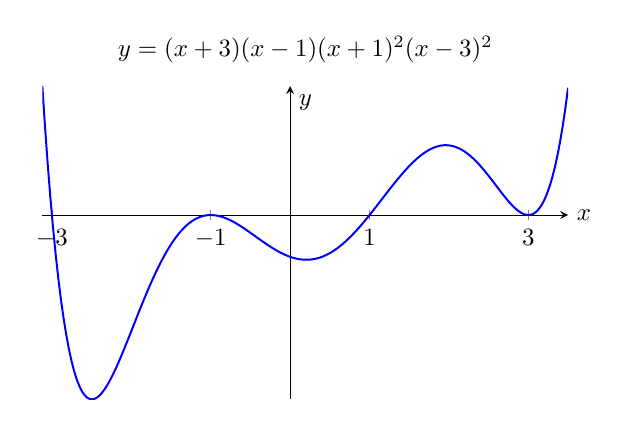
\begin{tikzpicture}[scale=0.9]
  \begin{axis} [
    width=9cm, height=6cm,
    axis lines=middle,
    xlabel={$x$}, xlabel style={right}, ylabel={$y$},
    xtick={-3,-1,1,3},
    xticklabels={$-3$,$-1$,$1$,$3$},
    ytick=\empty,
    domain=-3.12:3.5,
    samples=200,
    title={$y = (x+3)(x-1)(x+1)^2(x-3)^2$}
  ]
    % Đồ thị hàm số mới
    \addplot[blue, thick] {(x+3)*(x-1)*(x+1)^2*(x-3)^2};
    % Đánh dấu nghiệm bằng vạch dọc trên trục hoành
    % Không cần addplot marks nữa, chỉ dùng xtick
  \end{axis}
\end{tikzpicture}
\end{center}
% --- Hết đồ thị minh họa ---
\end{banchat}

\end{lythuyetbox}

\section{Một số hàm số thường gặp}
\begin{lythuyetbox}{Hàm số bậc ba}

  % --- Lý thuyết về hàm số bậc ba ---
  Hàm số bậc ba có dạng:
  \[ y = ax^3 + bx^2 + cx + d \]
  Đạo hàm:
  \[ y' = 3a x^2 + 2b x + c \]
  Khi này, ta xét tam thức bậc hai
  \begin{itemize}
      \item $y' \geq 0,\ \forall x \in \mathbb{R} \Leftrightarrow \begin{cases} a > 0 \\ \Delta \leq 0 \end{cases}$
      \item $y' \leq 0,\ \forall x \in \mathbb{R} \Leftrightarrow \begin{cases} a < 0 \\ \Delta \leq 0 \end{cases}$ 
  \end{itemize}
  Bổ sung: $y' \neq 0$ với mọi $x$ khi $\Delta \neq 0$ (vì nó có nghiệm)

  \vspace{1.5em}
  Cực trị:
  \begin{itemize}
      \item 2 cực trị $\Leftrightarrow \Delta > 0$ (có 2 nghiệm phân biệt)
      \item Không có cực trị $\Leftrightarrow$
      $\left\{\begin{array}{l}
          \Delta < 0 \quad \text{(không có nghiệm)} \\
          \Delta = 0 \quad \text{(có nghiệm kép)}
      \end{array}\right.$
  \end{itemize}

\end{lythuyetbox}

\begin{lythuyetbox}{Hàm phân thức bậc nhất/bậc nhất}
  Hàm phân thức bậc nhất có dạng:
  \[ y = \frac{ax + b}{cx + d} \qquad (x \neq -\frac{d}{c}) \]
  Đạo hàm:
  \[ y' = \frac{ad-bc}{(cx + d)^2} \]
  Từ đây, với $ad - bc$ là hằng số, dễ dàng suy ra rằng:
  \begin{itemize}
      \item Nếu $ad - bc > 0$ thì $y' > 0$, hàm đồng biến trên khoảng xác định.
      \item Nếu $ad - bc < 0$ thì $y' < 0$, hàm nghịch biến trên khoảng xác định.
      \item Nếu $ad - bc = 0$ thì $y' = 0$, hàm không đổi trên khoảng xác định.
  \end{itemize}

\end{lythuyetbox}

\begin{lythuyetbox}{Hàm trùng phương}
  Hàm trùng phương có dạng:
\[
    y = ax^4 + bx^2 + c
\]
Đạo hàm:
\[
    y' = 4a x^3 + 2b x = 2x(2a x^2 + b)
\]
\[
    y' = 0 \Leftrightarrow
    \left[\begin{array}{l}
        x = 0 \\  x^2 = -\dfrac{b}{2a}
    \end{array}\right.
\]
\textbf{Các trường hợp:}

\[
\left.\begin{aligned}
    &\text{TH1:}\quad b = 0 \Rightarrow x^2 = 0 \Rightarrow x = 0 \text{ là nghiệm bội ba (lẻ)} \\
    &\text{TH2:}\quad -\dfrac{b}{2a} < 0 \Leftrightarrow ab > 0 \Rightarrow x^2 = -\dfrac{b}{2a} \text{ vô nghiệm}
\end{aligned}\right\}
\Rightarrow \textbf{0 là cực trị duy nhất}
\]

\[
\text{TH3:}\quad -\dfrac{b}{2a} > 0 \Leftrightarrow ab < 0 \Rightarrow x^2 = -\dfrac{b}{2a} \text{ có hai nghiệm phân biệt } x = \pm \sqrt{-\dfrac{b}{2a}}
\]
\qquad $\Rightarrow$ Hàm số có 3 cực trị

\vspace{1.5em}
\textbf{Kết luận:}
\begin{itemize}
    \item Hàm trùng phương có 1 cực trị $\iff ab \geq 0$
    \item Hàm trùng phương có 3 cực trị $\iff ab < 0$
    \item Trong cả hai trường hợp đều có $x = 0$ là cực trị.
\end{itemize}

\textbf{Tính chất của 3 điểm cực trị:}

Với hàm số $y = f(x) = ax^4 + bx^2 + c$ (với $ab < 0$ để có 3 cực trị), ta có:

\begin{itemize}
    \item Ba điểm cực trị là $x_1 = 0$, $x_2 = \sqrt{-\dfrac{b}{2a}}$, $x_3 = -\sqrt{-\dfrac{b}{2a}}$.
    \item Giá trị hàm số tại hai điểm đối xứng:
    \[
        f\left(\sqrt{-\dfrac{b}{2a}}\right) = f\left(-\sqrt{-\dfrac{b}{2a}}\right)
    \]
    \item Ba điểm cực trị tạo thành các đỉnh của một tam giác cân trên mặt phẳng tọa độ.
\end{itemize}

\begin{center}
\begin{tikzpicture}[scale=1.1]
  % Trục toạ độ
  \draw[->] (-2.2,0) -- (2.2,0) node[right] {$x$};
  \draw[->] (0,-0.5) -- (0,3.2) node[above] {$y$};
  % Các điểm cực trị minh hoạ với a=1, b=-2, c=0
  \coordinate (A) at (0, 1);
  \coordinate (B) at (1, -1);
  \coordinate (C) at (-1, -1);
  % Vẽ tam giác
  \draw[thick, blue] (A) -- (B) -- (C) -- cycle;
  % Đánh dấu các điểm
  \filldraw[red] (A) circle (2pt) node[above right] {$A(0,\ c)$};
  \filldraw[red] (B) circle (2pt) node[below right] {$B(x_2,\ y_2)$};
  \filldraw[red] (C) circle (2pt) node[below left] {$C(x_3,\ y_3)$};
  % Ghi chú
  \node at (0,2.5) {\footnotesize Tam giác cân tại $A$};
\end{tikzpicture}
\end{center}

\end{lythuyetbox}